\documentclass[UTF8]{article}
\usepackage[fontset=fandol]{ctex} % Chinese support, using Fandol fonts
\usepackage{graphicx} % Insert images
\usepackage{listings} % Print source code
\usepackage{xcolor} % Color support
\usepackage{booktabs} % Professional table support
\usepackage{pdflscape} % Landscape pages support in PDF
\usepackage{hyperref} % Hypertext links support for cross-referencing
\usepackage{geometry}
\usepackage{enumitem}
\usepackage{setspace}

% Customize hyperref format (it's set to no special format here)
\hypersetup{hidelinks}

% Declare directories to search for graphics files for graphicx
\graphicspath{{figures/}}

% Define source code style for listings
\lstdefinestyle{c-style}{
  language=C,
  basicstyle=\ttfamily\small\fontfamily{pcr}\selectfont, % 使用 Courier New 字体
  keywordstyle=\bfseries\color{blue},
  identifierstyle=\color{black},
  stringstyle=\color{red},
  commentstyle=\itshape\color{gray},
  backgroundcolor=\color{gray!3},
  numbers=left,
  numberstyle=\tiny\color{gray},
  numbersep=8pt,
  breaklines=true,
  postbreak=\mbox{\textcolor{red}{$\hookrightarrow$}\space},
  frame=single,
  framerule=0.5pt,
  rulecolor=\color{black},
  tabsize=4,
  captionpos=b,
  xleftmargin=15pt,
  xrightmargin=15pt,
  aboveskip=10pt,
  belowskip=10pt,
  showspaces=false,
  showstringspaces=false,
  showtabs=false,
  morekeywords={*,printf,scanf},
  escapeinside={(*@}{@*)}, % 支持代码中插入LaTeX
}

% Define new command for title page
\newcommand{\reporttitle}[2]{
  \LARGE\textsf{#1}\quad\underline{\makebox[12em]{#2}}
}
\newcommand{\reportinfo}[2]{
  \large\makebox[4em]{\textsf{#1}}\quad\underline{\makebox[18em]{#2}}
}

% ----- The document begins here -----
\begin{document}

% Title page
\title{\Huge Hajimi-OS 作品文档}
\author{夏彦文 \thanks{学生,计算机学院数据科学与大数据} \and 雷翔麟 \thanks{学生,计算机科学与技术学院}
  \and 邹扬 \thanks{学生,计算机学院数据科学与大数据} \and 潘鹏 \thanks{指导教师,计算机科学与技术学院}}
\date{\today}
\maketitle

% Table of contents
\newpage
\tableofcontents
\newpage

% 设定1.6倍行距
\setstretch{1.6}

% Main content
\section{作品介绍}
\subsection{项目背景及意义}
\subsection{国内外研究状况}
\subsection{项目的主要工作}

\section{目标理念}

\section{系统设计与实现}
\subsection{进程管理}
进程管理模块的主要功能包括:初始化进程、加载和解析进程、切换进程,以及构建进程状态模块。具体功能介绍如下。
\subsubsection{进程控制块}
进程作为操作系统提供的一种抽象层,实际上代表了正在执行的程序。为了便于管理进程,\texttt{Hajimi-OS}采用进程控制块\texttt{PCB}来管理操作系统的进程。进程控制块的结构如下所示。
进程控制块中包含了进程的状态信息,这是操作系统管理进程的基本单元。关于具体的状态,我们将在后文详细解析。
\lstinputlisting[style=c-style]{processblock.c}
\subsubsection{进程状态}
进程状态是一个枚举类型,其定义如下:
\lstinputlisting[style=c-style]{processstate.c}
各状态对应如下:
\begin{enumerate}[label=\textbf{\arabic*}., wide, labelwidth=!, labelindent=0pt]
  \item UNUSED 状态表示进程控制块未关联任何进程。
  \item SLEEPING 状态表示进程因某种原因暂时未运行。
  \item RUNNABLE 状态表示进程正等待调度器安排运行
  \item RUNNING 状态表示进程正在执行中。
  \item ZOMBIE 状态表示进程已终止,但资源尚未被回收。
\end{enumerate}
\subsubsection{分配进程}
在 \texttt{Hajimi-OS} 中,分配新进程的过程由 \texttt{allocproc} 函数负责。这个函数主要执行以下步骤:
\begin{enumerate}[label=\textbf{\arabic*}., wide, labelwidth=!, labelindent=0pt]
  \item \textbf{查找 UNUSED 状态的进程控制块:} 系统首先会扫描进程控制块数组,寻找一个状态为 \texttt{UNUSED} 的控制块。如果找到,程序跳转到 \texttt{found} 标签继续操作;如果未找到,则返回 \texttt{NULL},表示当前没有可用的进程控制块,无法创建新进程。
  \item \textbf{初始化进程控制块:} 找到未使用的进程控制块后,函数会分配一个新的进程 ID(通过调用 \texttt{allocpid} 函数),将虚拟内存地址\texttt{vma}设置为 \texttt{NULL},并将内核时间\texttt{ktime}和用户时间\texttt{utime}初始化为 1。
  \item \textbf{分配 trapframe 页面:} 函数为新进程的 \texttt{trapframe} 分配内存(通过调用 \texttt{kalloc} 函数)。如果内存分配失败,函数将释放进程锁并返回 \texttt{NULL}。
  \item \textbf{创建用户和内核页表:} 成功分配 trapframe 页面后,函数创建一个空的用户页表(通过调用 \texttt{proc\_pagetable} 函数)和一个内核页表(通过调用 \texttt{proc\_kpagetable} 函数)。如果任一页表创建失败,函数会清理进程资源并返回 \texttt{NULL}。
  \item \textbf{配置内核堆栈\texttt{kstack}:} 成功分配页表后,函数会设置进程的内核堆栈地址,该地址是预设的虚拟地址。
  \item \textbf{设置新进程的上下文:} 函数初始化进程的上下文\texttt{context},将返回地址寄存器\texttt{ra}设为 \texttt{forkret} 函数地址,堆栈指针\texttt{sp}设为内核堆栈顶部。如此设置后,新进程将从 \texttt{forkret} 函数开始执行。
\end{enumerate}
通过这些步骤,\texttt{allocproc} 函数完成了新进程的创建。每个新创建的进程在完成这些步骤后,都会拥有一个唯一的进程 \texttt{ID},以及自己的页表和堆栈,准备好开始执行。
\subsubsection{加载和解析进程}
在 \texttt{Hajimi-OS} 中,除 \texttt{init} 进程外,所有进程都是通过 \texttt{fork} 系统调用进行复制,然后使用 \texttt{exec} 系统调用加载新程序来执行的。
对于 \texttt{init} 进程,初始化过程如下:
\begin{enumerate}[label=\textbf{\arabic*}., wide, labelwidth=!, labelindent=0pt]
  \item \textbf{进程分配:} \texttt{Hajimi-OS} 预设了固定数量的进程控制块 \texttt{Process Control Block}。每次创建新进程时,系统会在 \texttt{PCB} 数组中寻找一个空闲的块。
  \item \textbf{页表映射:} \texttt{Hajimi-OS} 使用 \texttt{RISC-V} 的 \texttt{sv39} 虚拟内存模型。在此步骤中,操作系统会为程序的各个段(如代码段、数据段等)进行页表映射。我们预先编译了一段二进制代码,专门用于执行 \texttt{init} 程序。 \texttt{init} 程序将使用 \texttt{fork} 系统调用创建一个新进程,然后通过 \texttt{exec} 系统调用执行 \texttt{shell} 程序。原始的 \texttt{init} 进程则会进入无限的进程调度循环。
  \item \textbf{设置进程状态:} 完成以上步骤后,操作系统将进程状态设置为 \texttt{RUNNABLE}。
\end{enumerate}
代码如下:
\lstinputlisting[style=c-style]{processinit.c}
对于其他进程,其初始化过程大致如下:
\begin{enumerate}[label=\textbf{\arabic*}., wide, labelwidth=!, labelindent=0pt]
  \item \textbf{使用 \texttt{fork} 系统调用:} \texttt{fork} 的主要功能是生成一个与父进程完全相同的子进程。这个过程包括为新进程创建一个进程控制块\texttt{PCB},复制父进程的页表,并在 \texttt{PCB} 中记录父子进程关系,具体存储在 \texttt{PCB} 的 \texttt{parent} 字段中。
  \item \textbf{执行 \texttt{exec} 系统调用:} \texttt{exec} 的主要作用是解析 \texttt{ELF} 文件,并为进程重新映射虚拟内存。通过这种方式,新程序能够在原进程的环境中运行,而不仅仅是复制父进程的行为。这个过程确保了进程的正确创建和程序的正确加载,保证了 \texttt{Hajimi-OS} 的多进程环境能够正常运行。
\end{enumerate}

\subsubsection{进程调度}
目前,texttt{Hajimi-OS} 操作系统采用时间片均分策略进行进程调度。因此,在时钟中断时,操作系统会中断当前进程并调度下一个进程执行。所有进程的优先级相同,统一放在一个队列中进行调度。接下来,我们将介绍进程切换过程,但首先需要了解 Hajimi-OS 对 CPU 的抽象。

在 \texttt{Hajimi-OS} 中,\texttt{CPU} 由以下结构体管理,其中关键字段是 \texttt{proc} 和 \texttt{context}。\texttt{proc} 字段指向当前在该 \texttt{CPU} 上运行的进程,而 \texttt{context} 字段用于进程切换。
\lstinputlisting[style=c-style]{cpustruct.c}
context 的定义如下:
\lstinputlisting[style=c-style]{contextstruct.c}
context 用于保存当前进程的上下文,以便进程下次运行时恢复。Hajimi-OS 的进程调度通过 \texttt{scheduler} 函数实现,当系统需要进行进程切换时,它会扫描所有进程,寻找状态为 RUNNABLE 的进程。

首先,\texttt{scheduler} 函数从进程列表中选择一个状态为 RUNNABLE 的进程。获取进程后,会锁定该进程以防止其他进程同时修改其状态。

接下来,将选中的 RUNNABLE 进程状态改为 RUNNING,并将其设置为当前 CPU 正在运行的进程。此时,函数会切换页表到选中进程的内核页表,并刷新地址空间。

然后,函数执行 \texttt{swtch} 操作,将当前 CPU 的 context 与待运行进程的 context 进行切换。此操作涉及更改处理器的 ra 和 sp 寄存器,使处理器跳转到新进程指定的地址执行,即待运行进程的 ra 寄存器地址。当进程运行结束后,处理器会返回到 \texttt{scheduler} 函数,并将页表切换回内核页表,同时刷新地址空间。此时,进程状态可能已发生变化。

最后,当前 CPU 的正在运行进程被设置为 0,表示 CPU 暂时没有正在运行的进程。然后释放进程的锁,进行下一轮进程选择。

如果在一轮循环中没有找到可运行的进程,系统将执行 \texttt{wfi} 指令使处理器进入休眠状态,等待中断唤醒。

\subsubsection{进程释放}
在 Hajimi-OS 中,当一个进程结束或在进程创建过程中发生错误时,需要释放该进程所占用的资源,这个过程通过 freeproc 函数来完成。该函数的主要步骤如下:
\begin{enumerate}[label=\textbf{\arabic*}., wide, labelwidth=!, labelindent=0pt]
  \item \textbf{释放 \texttt{trapframe}:} 首先,如果 \texttt{trapframe} 存在,则释放其占用的内存,并将 \texttt{trapframe} 字段设为 0。
  \item \textbf{释放内核页表:} 如果内核页表\texttt{kpagetable}存在,则释放其占用的内存,然后将 \texttt{kpagetable} 字段设为 0。
  \item \textbf{释放用户页表:} 如果用户页表\texttt{pagetable}存在,利用 \texttt{proc\_freepagetable} 函数释放用户页表所占用的内存,同时将 \texttt{pagetable} 字段设为 0。
  \item \textbf{清空进程控制块的其他字段:} 清空进程的虚拟内存地址\texttt{vma},将进程大小\texttt{sz}设为 0,进程 ID\texttt{pid}设为 0,父进程\texttt{parent}设为 0,清空进程的名称\texttt{name},清空等待的条件变量\texttt{chan},设置进程未被杀死(将 \texttt{killed} 设为 0),并将进程的扩展状态设为 0。
  \item \textbf{设置进程状态为 \texttt{UNUSED}:} 最后,将进程状态设为 \texttt{UNUSED},表示该进程控制块可以重新分配给新的进程使用。
\end{enumerate}
通过这些步骤,\texttt{freeproc} 函数实现了对进程资源的回收,包括内存资源(如 trapframe、页表等)和进程控制块中的各种字段。回收完毕后,该进程控制块即可被系统重新利用,用于创建新的进程。

\subsection{内存管理}
\subsubsection{物理内存管理}
物理内存管理是操作系统的核心部分之一。Hajimi-OS 采用了一种简单且高效的物理内存分配和回收算法,主要由 kalloc.c 模块负责。该模块实现了初始化物理内存、分配物理内存和回收物理内存的功能。

\paragraph{内存管理概述\\}
在 Hajimi-OS 中,物理内存是按页进行管理的,每页大小为 4096 字节。系统中的所有空闲物理内存页通过一个单向链表组织起来,链表中的每个节点代表一个物理内存页。以下是相关数据结构和变量:
\begin{enumerate}[label=\textbf{\arabic*}., wide, labelwidth=!, labelindent=0pt]
  \item \textbf{struct run}: 这是一个简单的链表节点结构,表示一个空闲的物理内存页,next 指针指向下一个空闲内存页。
        \lstinputlisting[style=c-style]{runstruct.c}
  \item \textbf{kmem}: 这是一个全局变量,用于管理所有的空闲物理内存页。texttt{freelist} 指针指向空闲内存页链表的头部,\texttt{npage} 记录当前系统中空闲物理内存页的数量。\texttt{kmem} 中还包含一个名为 \texttt{lock} 的自旋锁,用于在多核环境下保护内存分配和回收操作的原子性。
        \lstinputlisting[style=c-style]{kmemstruct.c}
\end{enumerate}

\paragraph{核心函数}
\begin{enumerate}[label=\textbf{\arabic*}., wide, labelwidth=!, labelindent=0pt]
  \item \texttt{kfree} 该函数用于释放一个物理内存页,接收一个指向物理内存页的指针。函数首先检查传入的物理地址是否合法,然后将该物理内存页的内容清空,并将其添加到空闲内存页链表的头部。
  \lstinputlisting[style=c-style]{kfree.c}
  \item \texttt{kalloc} 该函数用于释放一个物理内存页,接收一个指向物理内存页的指针。函数首先检查传入的物理地址是否合法,然后将该物理内存页的内容清空,并将其添加到空闲内存页链表的头部。
  \lstinputlisting[style=c-style]{kalloc.c}
  \item \texttt{kinit} 该函数在系统启动时调用,用于初始化物理内存管理系统。它首先初始化 \texttt{kmem} 中的自旋锁,然后调用 \texttt{freerange} 函数,将从内核结束地址 \texttt{kernel\_end} 到物理内存上限 \texttt{PHYSTOP} 之间的所有物理内存页添加到空闲列表中。
  \lstinputlisting[style=c-style]{kinit.c}
  \item \texttt{freerange} 此函数用于将一段物理内存地址范围内的所有物理内存页释放,并加入到空闲内存页链表中。它首先将起始地址向上取整到页的边界,然后从起始地址开始,每次增加一个页的大小(4096 字节),依次释放每个物理内存页。
  \lstinputlisting[style=c-style]{freerange.c}
  \item \texttt{freemem\_amount} 此函数返回当前系统中的空闲物理内存量。由于内存页的大小是固定的,所以直接将空闲内存页的数量左移 12 位即可得到空闲内存的字节数。
  \lstinputlisting[style=c-style]{freemem_amount.c}
\end{enumerate}


\paragraph{设计评价与改进方向\\}
Hajimi-OS 的物理内存管理通过单一链表管理所有空闲内存页,采用简单的链表操作实现物理内存页的分配和回收,满足了操作系统对物理内存管理的基本需求。然而,未来可以考虑以下改进方向:
\begin{enumerate}[label=\textbf{\arabic*}., wide, labelwidth=!, labelindent=0pt]
  \item \textbf{支持大页分配:} 当前实现只支持分配和回收固定大小的内存页。如果需要分配大块的连续物理内存,需要进行多次分配操作,可能影响性能。可以考虑支持大页的分配,以提高内存访问的性能。
  \item \textbf{改进内存分配策略:} 目前的实现采用简单的“先进先出”策略分配内存页,可能导致物理内存的使用分布不均。可以考虑引入更复杂的内存分配策略,如伙伴系统(\texttt{Buddy System})或者 \texttt{slab} 分配器。
  \item \textbf{改进锁机制:} 当前实现中,所有对物理内存的操作都需要获取全局的 \texttt{kmem} 锁,这在多核环境下可能成为性能瓶颈。可以考虑引入更细粒度的锁机制,如每个 \texttt{CPU} 拥有自己的内存池和锁,或者使用无锁数据结构来提高并发性。
\end{enumerate}

\subsubsection{虚拟内存管理}

\paragraph{\texttt{Hajimi-OS} 虚拟内存管理\\}
页表是虚拟内存管理的重要工具。在 Hajimi-OS 中,运行在 RISC-V 的 Sv39 配置下,这意味着在 64 位虚拟地址中,只有低 39 位被使用,高 25 位闲置。Sv39 模式下,RISC-V 页表在逻辑层面上看似包含 2\textsuperscript{27} 个页表条目 PTE。每个 PTE 由 44 位的物理页码 PPN 和若干标志位组成。分页硬件利用虚拟地址的前 27 位索引页表,生成的物理地址为 56 位,其前 44 位来自 PTE 中的 PPN,后 12 位直接来自虚拟地址。

\paragraph{页表结构与地址转换\\}
页表逻辑上是一个简单的 PTE 数组(见图 3.2)。页表允许操作系统控制虚拟地址到物理地址的映射,以 4096 字节(2\textsuperscript{12} 字节)为单位。在 Sv39 配置下,虚拟地址的前 25 位不参与地址转换;未来 RISC-V 设计中,这些位可能用于更多级别的地址转换。此外,物理地址的扩展空间也预留了 10 位以便扩展物理地址长度。基于技术预测,2\textsuperscript{39} 字节(512GB)的虚拟内存空间能满足 RISC-V 计算机应用的需求,物理内存空间的 2\textsuperscript{56} 字节也足以支持未来的 I/O 设备和 DRAM 需求。

地址转换是一个三步过程。页表在物理内存中以三层树状结构存储,根节点为一个 4096 字节的页表页面,包含 512 个 PTE。每个 PTE 记录了下一层页表页的物理地址。分页硬件依次利用虚拟地址的 27 位选择 PTE:前 9 位用于根页表页面,中间 9 位用于中间页表页面,最后 9 位用于最终页表页面。若缺少任何一个必要的 PTE,分页硬件会抛出页面错误异常,Hajimi-OS 负责处理该异常。

\paragraph{页表条目 PTE 与硬件缓存\\}
三级设计在许多虚拟地址范围未映射的情况下节省内存。例如,一个应用程序仅使用一个页面,顶级页目录仅使用第 0 个条目,忽略第 1 到第 511 个条目,无需为这些条目分配中级和低级页表页。该设计在这种情况下仅占用三个页面,总共 3 × 4096 字节。然而,CPU 在执行地址转换时必须从内存中提取三个 PTE,从而增加了内存访问的开销。为降低 PTE 加载成本,RISC-V CPU 将页表条目缓存在 Translation Look-aside Buffer中。

每个 PTE 包含若干标志位,指示分页硬件如何处理对应的虚拟地址:
\begin{enumerate}[label=\textbf{\arabic*}., wide, labelwidth=!, labelindent=0pt]
  \item PTE\_V:PTE 是否存在,未设置则引用页面引发异常。
  \item PTE\_R:是否允许读取页面。
  \item PTE\_W:是否允许写入页面。
  \item PTE\_X:是否允许执行页面内容。
  \item PTE\_U:用户模式下是否可访问页面。
\end{enumerate}
\lstinputlisting[style=c-style]{riscv.c}
这些标志位和结构在 \texttt{kernel\textbackslash include\textbackslash sys\textbackslash riscv.h} 中定义。

\paragraph{\texttt{Hajimi-OS} 虚拟内存管理代码\\}
虚拟内存管理系统主要负责分页和内存映射。关键函数包括:
\begin{enumerate}[label=\textbf{\arabic*}., wide, labelwidth=!, labelindent=0pt]
  \item \textbf{\texttt{kvminit()}:} 创建一个直接映射的页表用于内核,设置不同设备和内核区域的映射。
  \item \textbf{\texttt{kvminithart()}:} 设置硬件的页表寄存器为内核页表并启用分页。
  \item \textbf{\texttt{walk()}:} 返回对应给定虚拟地址的 PTE 地址,必要时创建页表页。
  \item \textbf{\texttt{walkaddr()}:} 返回给定虚拟地址对应的物理地址,未映射则返回 0。
  \item \textbf{\texttt{kvmmap()}:} 向内核页表添加映射,用于启动时,不刷新 TLB。
  \item \textbf{\texttt{kvmpa()}:} 将内核虚拟地址转换为物理地址,用于栈地址。
  \item \textbf{\texttt{mappages()}:} 创建页表条目,映射从 \texttt{va} 开始的虚拟地址到 \texttt{pa} 开始的物理地址。
  \item \textbf{\texttt{vmunmap()}:} 移除从 \texttt{va} 开始的 \texttt{npages} 页的映射,必要时释放物理内存。
  \item \textbf{\texttt{uvmcreate()}:} 创建空用户页表,内存不足时返回 0。
  \item \textbf{\texttt{uvminit()}:} 将用户初始代码加载到页表地址 0,用于第一个进程。
  \item \textbf{\texttt{uvmalloc1()}:} 虚拟地址 \texttt{start} 到 \texttt{end} 分配 PTE 和物理内存,成功返回 0 失败返回 -1。
  \item \textbf{\texttt{freewalk()}:} 遍历页表并递归释放所有子页表。
  \item \textbf{\texttt{uvmfree()}:} 释放用户内存页和页表页。
  \item \textbf{\texttt{uvmcopy()}:} 复制父进程页表及其物理内存到子进程页表。
  \item \textbf{\texttt{uvmclear()}:} 将指定虚拟地址的页表条目标记为用户无法访问。
  \item \textbf{\texttt{copyout()}:} 从内核复制数据到用户空间。
  \item \textbf{\texttt{copyout2()}:} 简化版 \texttt{copyout},直接在虚拟地址空间操作。
  \item \textbf{\texttt{copyin()}:} 从用户空间复制数据到内核。
  \item \textbf{\texttt{copyin2()}:} 简化版 \texttt{copyin},直接在虚拟地址空间操作。
  \item \textbf{\texttt{copyinstr()}:} 从用户空间复制以 null 结尾的字符串到内核空间。
  \item \textbf{\texttt{copyinstr2()}:} 简化版 \texttt{copyinstr},直接在虚拟地址空间操作。
  \item \textbf{\texttt{proc\_kpagetable()}:} 初始化每个进程的内核页表。
  \item \textbf{\texttt{kfreewalk()}:} 释放页表的内核空间。
  \item \textbf{\texttt{kvmfreeusr()}:} 释放用户页表的内核空间。
  \item \textbf{\texttt{kvmfree()}:} 释放整个内核页表。
  \item \textbf{\texttt{vmprint()}:} 打印页表的详细信息。
  \item \textbf{\texttt{experm()}:} 改变指定虚拟地址的页表条目的权限。
\end{enumerate}

\paragraph{虚拟内存管理设计\\}
\texttt{Hajimi-OS} 的分页系统将物理内存和虚拟内存划分为固定大小的页,通过页表进行映射。页表条目包含页的权限标志位和物理地址。多个函数用于遍历和修改页表,例如 \texttt{walk} 函数查找特定 \texttt{PTE},\texttt{mappages} 函数修改页表以映射虚拟地址到物理地址。\texttt{freewalk} 函数递归释放页表页,\texttt{uvmfree} 函数释放用户内存页和页表页。\texttt{uvmcopy} 负责从父进程页表复制内存到子进程页表,实现进程创建。\texttt{copyin} 和 \texttt{copyout} 实现内核与用户空间之间的数据复制。\texttt{experm} 函数修改页表条目的权限,\texttt{vmunmap} 函数取消页表中虚拟地址的映射。

\texttt{Hajimi-OS} 进程拥有独立页表,映射其虚拟地址空间到物理内存。操作系统在进程切换时也会切换页表,确保正确的地址映射。每个进程的用户内存从虚拟地址 \texttt{0} 开始,可增长至 \texttt{MAXVA}(定义于 \texttt{riscv.h}),内存寻址空间可达 \texttt{256GB}。独立页表和虚拟地址空间切换实现了进程隔离和内存地址映射,确保每个进程拥有独立的内存空间,同时提供灵活性和可扩展性,满足不同应用需求。

当进程请求更多用户内存时,\texttt{Hajimi-OS} 首先使用 \texttt{kalloc} 分配物理页面,再将相应的 \texttt{PTE} 添加到进程页表中,指向新分配的物理页面,并设置 \texttt{PTE} 标志位以指示页面的读写、执行和用户访问权限。大多数进程不使用整个用户地址空间,\texttt{Hajimi-OS} 在未使用的页表项中将 \texttt{PTE\_V} 标志设置为空闲状态。

页表的典型使用示例包括:不同进程的页表将用户地址转换为不同物理内存页面,使每个进程拥有独立的私有内存空间;每个进程看到的用户内存空间以虚拟地址 0 开始,可为非连续的物理内存;内核在用户地址空间顶部映射一个包含蹦床代码的页面,使所有进程地址空间均可访问同一物理页面。

% 插入展示图片
\begin{figure}[htbp]
  \centering
  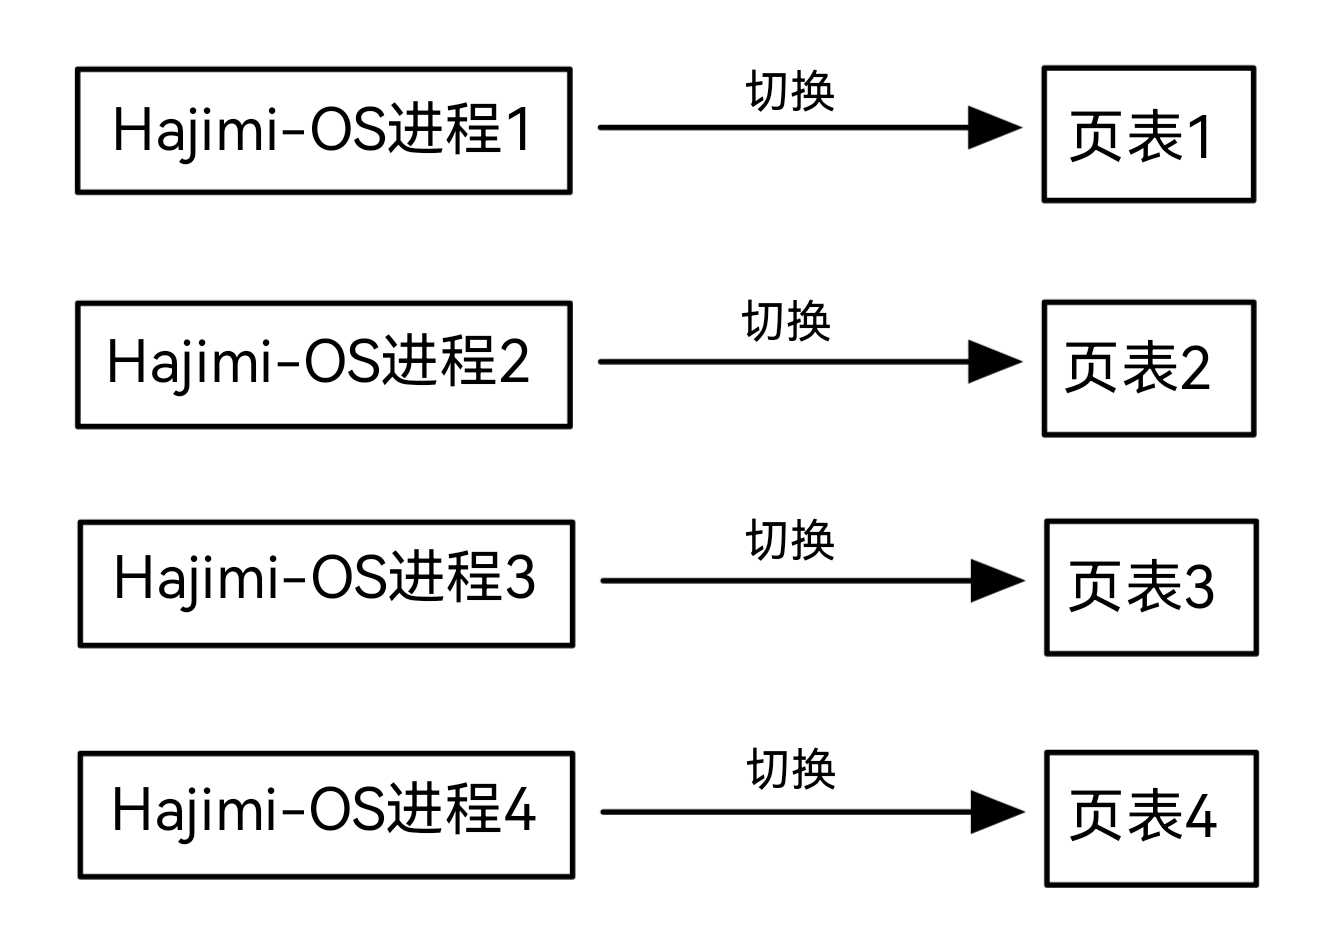
\includegraphics[width=0.8\textwidth]{mm1.png}
  \caption{进程页表}
  \label{进程页表}
\end{figure}
\begin{figure}[htbp]
  \centering
  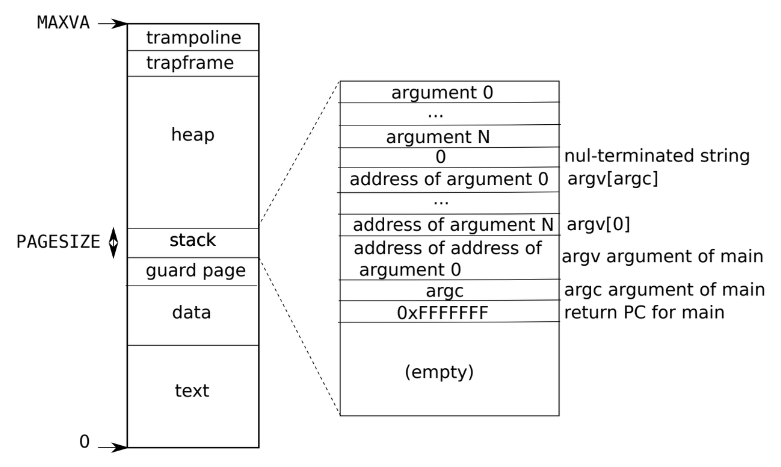
\includegraphics[width=0.8\textwidth]{mm2.png}
  \caption{地址空间}
  \label{地址空间}
\end{figure}

\paragraph{栈管理与保护\\}
在 Hajimi-OS 中,栈被分配为单独的页面,并在 \texttt{exec} 系统调用后初始化。栈的顶部包含命令行参数字符串及其指针数组,栈下方则包含启动程序所需的值,例如 \texttt{main} 函数的地址、\texttt{argc} 和 \texttt{argv} 参数。这样设计使程序如同刚刚调用 \texttt{main(argc, argv)} 一样开始执行。为了检测用户栈溢出,Hajimi-OS 在栈下方放置了一个无效的保护页(guard page)。如果用户栈溢出并尝试使用栈下方地址,由于该地址的页表项无效(\texttt{PTE\_V} 为 0),硬件会产生页面故障异常。当用户栈溢出时,操作系统可能会自动分配更多内存来避免问题。

\subsubsection{未来改进方向}
\paragraph{内存保护和安全性增强}
引入更多内存保护机制,以提高系统安全性
\begin{enumerate}[label=\textbf{\arabic*}., wide, labelwidth=!, labelindent=0pt]
  \item \textbf{内存隔离}: 确保不同进程间的内存隔离,防止越权访问。
  \item \textbf{内存清零}: 在内存释放或重分配时,将其内容清零,以防止数据泄露。
\end{enumerate}

\paragraph{高级内存管理功能}
为进一步优化内存使用,可以考虑引入高级内存管理技术
\begin{enumerate}[label=\textbf{\arabic*}., wide, labelwidth=!, labelindent=0pt]
  \item \textbf{\texttt{内存压缩:}} 通过压缩内存数据,提高内存利用率。
  \item \textbf{\texttt{NUMA 感知:}} 优化多处理器系统中的内存访问,以减少延迟。
  \item \textbf{\texttt{内存池预分配:}} 预先分配内存池以减少内存分配开销。
\end{enumerate}

\paragraph{增加缓存或预取机制}
通过预读取和缓存,提高内存访问速度
\begin{enumerate}[label=\textbf{\arabic*}., wide, labelwidth=!, labelindent=0pt]
  \item \textbf{\texttt{缓存机制:}} 在硬件或软件层面引入缓存,以减少内存访问延迟。
  \item \textbf{\texttt{预取机制:}} 提前加载可能会用到的数据,减少等待时间。
\end{enumerate}

\paragraph{增强错误处理}
设计更详细的错误处理机制
\begin{enumerate}[label=\textbf{\arabic*}., wide, labelwidth=!, labelindent=0pt]
  \item 当映射失败或访问权限违规时,提供明确的错误码和处理逻辑。
\end{enumerate}

通过以上改进,Hajimi-OS 可以进一步优化内存管理,提高系统性能和安全性,满足更复杂和多样化的应用需求。

\subsection{文件系统}

\section{系统调用的设计实现}

\section{系统测试}

\section{总结与展望}


% % Insert an image, with placement specifier htbp
% \begin{figure}[htbp]
%   \centering
%   
\includegraphics[width=0.5\textwidth]{JimMorhard}
%   \caption{Jim Morhard 演示立扫帚实验}
%   \label{JimMorhard}
% \end{figure}
% \subsection{扫帚的选择}
% 不同的扫帚参数各异,这里列出了部分扫帚的参数,请见表 \ref{broomsticks}。

% % Insert a three-line table
% \begin{table}[htbp]
%   \centering
%   \begin{tabular}{cccc}
%     \toprule
%     序号 & 名称 & 上市时间 & 最高时速 \\
%     \midrule
%     1 & 彗星290 & 1995年 & 60\,mph \\
%     2 & 光轮1000 & 1967年 & 100\,mph \\
%     3 & 光轮2001 & 1992年 & >\,100\,mph \\
%     4 & 火弩箭 & 1993年 & 150\,mph \\
%     \bottomrule
%   \end{tabular}
%   \caption{部分扫帚的参数对比}
%   \label{broomsticks}
% \end{table}
\end{document}
